\documentclass[11pt]{article}

\usepackage[a4paper,margin=1in]{geometry}
\usepackage{graphicx}
\usepackage{amsmath,amssymb}
\usepackage{booktabs}
\usepackage{siunitx}
\usepackage[colorlinks=true,linkcolor=blue!50!black,citecolor=blue!50!black,urlcolor=blue!50!black,
  pdftitle={Fluid Substitution and Pre-Stack Seismic Modeling},
  pdfauthor={Sumit},
  pdfsubject={Rock Physics and AVO Modeling Study},
  pdfkeywords={Gassmann fluid substitution, rock physics template, AVO, pre-stack seismic modeling}]{hyperref}
\usepackage{caption}
\usepackage{titlesec}
\usepackage{enumitem}
\usepackage{fancyhdr}
\usepackage{xcolor}

\graphicspath{{../figures/}}

\titleformat{\section}{\normalfont\Large\bfseries}{\thesection}{1em}{}
\titleformat{\subsection}{\normalfont\large\bfseries}{\thesubsection}{1em}{}

\pagestyle{fancy}
\fancyhf{}
\fancyhead[L]{\small Fluid Substitution \& Pre-Stack Seismic Modeling}
\fancyhead[R]{\small \thepage}
\renewcommand{\headrulewidth}{0.4pt}

\setlength{\parindent}{0pt}
\setlength{\parskip}{6pt}

\title{\Large\textbf{Fluid Substitution and Pre-Stack Seismic Modeling for\\
AVO-Based Fluid Discrimination in a Shaly-Sand Clastic Reservoir}\\[6pt]
\large A Rock-Physics and Quantitative Interpretation Study}
\author{Sumit}
\date{October 2025}

\begin{document}

\begin{titlepage}
\centering
\vspace*{2.5cm}
{\Huge\bfseries Fluid Substitution and Pre-Stack\\[4pt] Seismic Modeling\par}
\vspace{0.8cm}
{\Large AVO-Based Fluid Discrimination in a Shaly-Sand\\ Clastic Reservoir\par}
\vspace{1.2cm}
{\large\itshape A Rock-Physics and Quantitative Interpretation Study\par}
\vspace{2.5cm}
{\Large Sumit\par}
\vspace{0.4cm}
{\large October 2025\par}
\vfill
{\small Gassmann fluid substitution \(\cdot\) rock physics templates \(\cdot\) pre-stack AVO modeling\par}
\vspace{1cm}
\end{titlepage}

\section*{Abstract}
This study applies a rock-physics and quantitative-interpretation workflow to a synthetic, shaly-sand Tertiary clastic reservoir in order to predict the seismic amplitude-versus-offset (AVO) response to changes in pore fluid. Gassmann fluid substitution is used to transform an in-situ, brine-saturated reservoir sand into oil- and gas-charged equivalents, from which a Vp/Vs-versus-acoustic-impedance rock physics template is constructed and calibrated against synthetic well-log and core data. Pre-stack synthetic angle gathers, generated with a three-term linearized reflectivity approximation and a zero-phase wavelet, are used to classify the resulting AVO anomalies. The brine case yields a Class~I response, the oil case a notably subtle, near-zero-intercept Class~II/IIp response that requires full-angle gradient analysis to resolve, and the gas case an unambiguous Class~III bright-spot response. The workflow -- and every quantitative result reported below -- is fully reproducible from the accompanying source code.

\tableofcontents
\thispagestyle{empty}
\newpage

\section{Introduction and Objectives}

Discriminating pore fluid from lithology is one of the central problems in quantitative seismic interpretation. A change in pore fluid alters the bulk modulus of a reservoir rock while leaving its shear modulus essentially unchanged, and this asymmetry is what makes amplitude-versus-offset (AVO) analysis diagnostic: the intercept and gradient of the pre-stack reflection amplitude, taken together, can separate a fluid effect from a purely lithological one in a way that a post-stack amplitude alone cannot.

This study works through that diagnostic chain end to end for a single, representative reservoir interval:

\begin{enumerate}[label=(\roman*)]
\item build a physically consistent well-log model of a shaly-sand reservoir;
\item use Gassmann fluid substitution to predict how that sand's elastic properties change when it is charged with oil or gas instead of brine;
\item calibrate a rock physics template that generalizes this fluid sensitivity across a range of porosity, for lithofacies and fluid-type discrimination; and
\item forward-model the pre-stack seismic response of each fluid case, and classify the resulting AVO anomaly.
\end{enumerate}

No proprietary or measured field dataset is used at any stage. The well-log model is a synthetic "type well," built from standard, cited empirical and petrophysical relations and calibrated to parameter ranges that are typical of a shallow, high-porosity, under-compacted Tertiary clastic section (broadly representative of North Sea-type basins). This choice keeps every input transparent and reproducible, and lets the workflow focus on the physics of fluid substitution and AVO response rather than on well-specific data conditioning.

\section{Geological Setting and Synthetic Well Data}

The modelled section spans 2000--2200~m true vertical depth, representative of a normally pressured, moderately young (Tertiary) clastic basin. A single, 16~m-thick, high-net-to-gross reservoir sand is present from 2140--2156~m, embedded in a shale-dominated background that also contains two thin, non-reservoir silty streaks included for log realism but excluded from the fluid-substitution and AVO analysis.

Shale volume (\(V_\mathrm{sh}\)) follows a smooth, log-resolution-limited transition into and out of the reservoir sand, superimposed on a slowly varying regional background and a band-limited noise texture that mimics real wireline log character. Porosity follows an Athy's-law (Athy, 1930) exponential compaction trend, distinct for the sand and shale end-members and mixed according to \(V_\mathrm{sh}\):
\[
\phi(z) = \phi_0 \, e^{-c z},
\]
with \(\phi_{0,\mathrm{sand}} = 0.45\), \(c_\mathrm{sand} = 1.2\times10^{-4}\,\text{m}^{-1}\), \(\phi_{0,\mathrm{shale}} = 0.55\), \(c_\mathrm{shale} = 3.5\times10^{-4}\,\text{m}^{-1}\). This produces a clean reservoir-sand porosity of approximately 33--35\%, consistent with the very high porosities documented in young, shallow, poorly consolidated Tertiary sands.

In-situ pressure and temperature follow simple linear gradients appropriate to a normally pressured basin: a hydrostatic pressure gradient of 10.0~MPa/km, and a geothermal gradient of 30~\si{\celsius}/km from an 8~\si{\celsius} surface (mudline) temperature. At the reservoir midpoint (2148~m) this gives \(T \approx 72.4\)~\si{\celsius} and \(P \approx 21.5\)~MPa.

\begin{figure}[htbp]
\centering
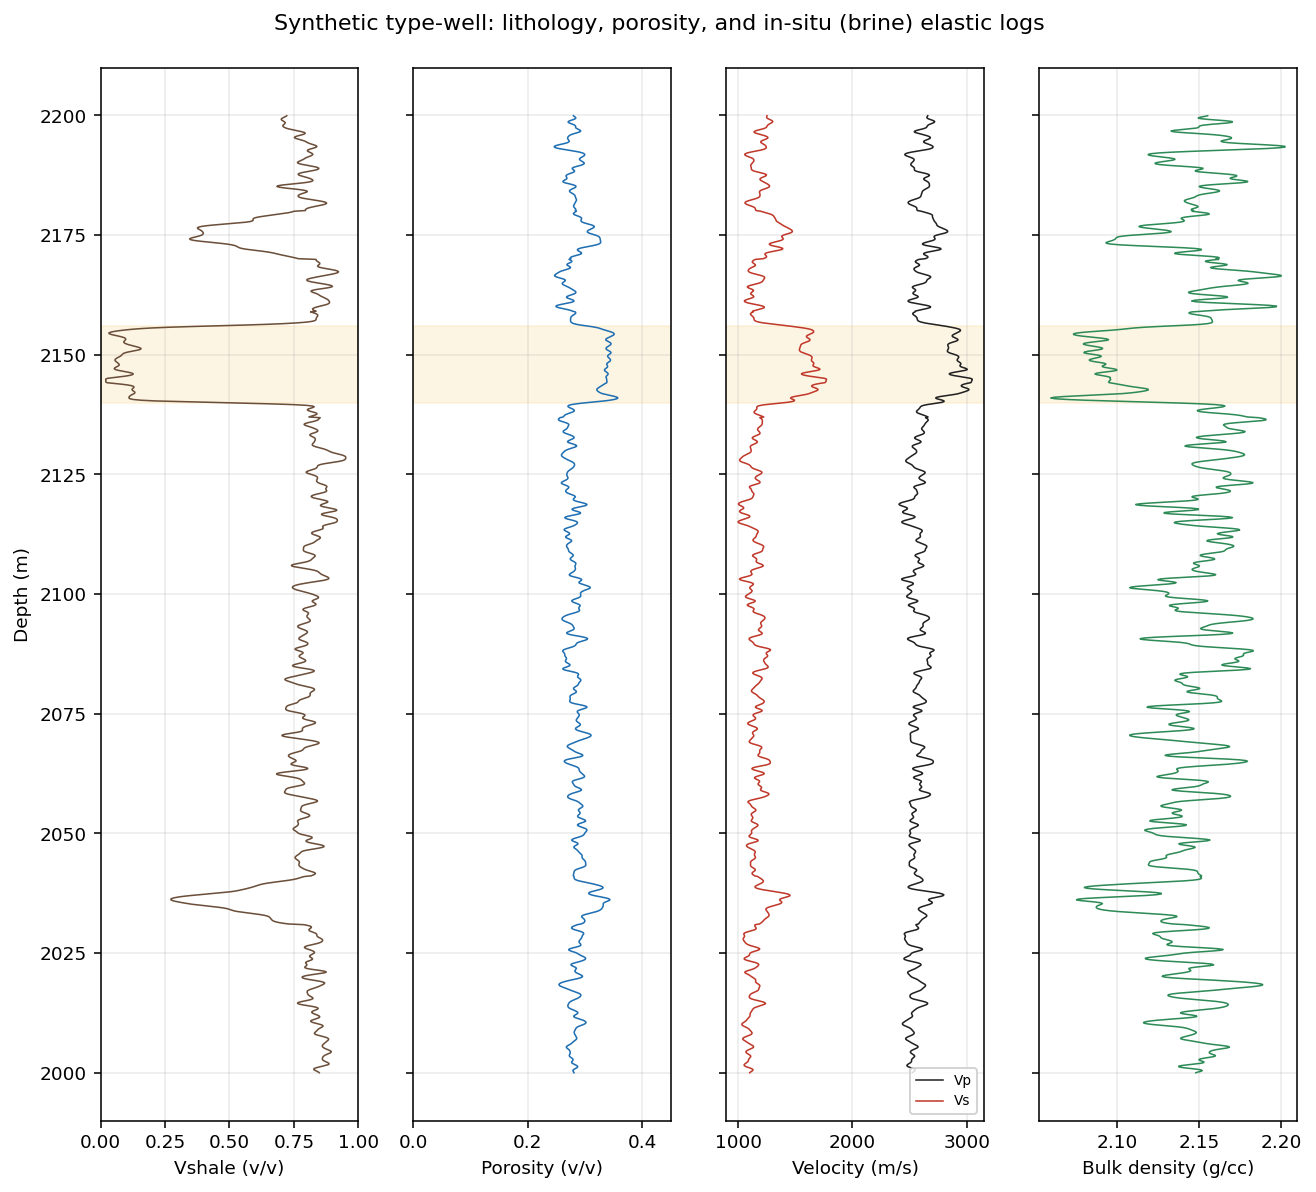
\includegraphics[width=0.95\textwidth]{01_log_tracks.png}
\caption{Synthetic type-well: lithology (Vshale), porosity, and in-situ (brine-saturated) Vp/Vs and bulk density logs. The reservoir interval (2140--2156~m) is highlighted.}
\label{fig:logs}
\end{figure}

\section{Methodology}

\subsection{Mineral and Fluid Properties}

Mineral moduli are computed as a Voigt-Reuss-Hill (Hill, 1952) average of quartz and clay end-members, weighted by \(V_\mathrm{sh}\):
\[
M_\mathrm{VRH} = \tfrac{1}{2}\left[ \left(f_1 M_1 + f_2 M_2\right) + \left( \frac{f_1}{M_1} + \frac{f_2}{M_2} \right)^{-1} \right],
\]
applied separately to the bulk (\(K\)) and shear (\(\mu\)) moduli, using \(K_\mathrm{qtz}=36.6\), \(\mu_\mathrm{qtz}=45.0\)~GPa, \(\rho_\mathrm{qtz}=2650\)~kg/m\(^3\) for quartz and \(K_\mathrm{clay}=20.9\), \(\mu_\mathrm{clay}=6.85\)~GPa, \(\rho_\mathrm{clay}=2580\)~kg/m\(^3\) for clay (representative literature values).

Brine density and acoustic velocity are computed with the Batzle \& Wang (1992) empirical relations (their eqs.~27b, 29), at 35{,}000~ppm NaCl salinity, using the open-source \texttt{bruges} rock-physics library's implementation. Oil is modelled as a dead (gas-free), 32\textdegree~API crude: density follows exactly from the API-gravity definition at stock-tank conditions, corrected to reservoir temperature and pressure with a simple linear thermal-expansion/compressibility relation, and combined with a representative reservoir-condition acoustic velocity (consistent with the range reported by Batzle \& Wang for a dead oil of this gravity) to obtain the bulk modulus. Gas is modelled under an ideal-gas approximation, consistent with the density relation used internally by the brine/gas routines this project depends on: \(\rho_g = MP/RT\) and an adiabatic bulk modulus \(K_g = \gamma P\), with an effective heat-capacity ratio \(\gamma=1.25\) representative of a light hydrocarbon gas. A full live-oil/real-gas PVT treatment (requiring measured GOR, bubble point, and gas composition) was not attempted, since no such measured PVT report exists for this synthetic case; this simplification is noted explicitly here and in the accompanying source code.

The resulting fluid properties at reservoir conditions (\(T=72.4\)\,\si{\celsius}, \(P=21.5\)~MPa) are summarized in Table~\ref{tab:fluids}.

\begin{table}[htbp]
\centering
\caption{Pore-fluid properties at in-situ reservoir conditions.}
\label{tab:fluids}
\begin{tabular}{lccc}
\toprule
Fluid & Density (kg/m\(^3\)) & Bulk modulus (GPa) & Basis \\
\midrule
Brine (35 kppm NaCl) & 1010 & 2.673 & Batzle \& Wang (1992) \\
Oil (32\textdegree~API, dead) & 840 & 1.577 & Simplified dead-oil PVT \\
Gas (\(\gamma_g=0.65\)) & 141 & 0.0269 & Ideal-gas approximation \\
\bottomrule
\end{tabular}
\end{table}

\subsection{Dry-Frame Rock Physics Model}

Dry-frame bulk and shear moduli are estimated with the Krief et al. (1990) relation, which links the frame moduli to the mineral moduli through porosity alone:
\[
\frac{K_\mathrm{dry}}{K_\mathrm{min}} = \frac{\mu_\mathrm{dry}}{\mu_\mathrm{min}} = (1-\phi)^{A/(1-\phi)}, \qquad A = 3.
\]
This model was chosen over a contact-cement or Hertz-Mindlin granular model because it requires no additional core-calibrated cementation or coordination-number parameters, which is appropriate for a first-pass, log-driven workflow of this kind.

\subsection{Gassmann Fluid Substitution}

Gassmann's (1951) equation relates the saturated-rock bulk modulus \(K_\mathrm{sat}\) to the dry-frame modulus \(K_\mathrm{dry}\), the mineral modulus \(K_\mathrm{min}\), the pore-fluid modulus \(K_\mathrm{fl}\), and porosity \(\phi\):
\[
K_\mathrm{sat} = K_\mathrm{dry} + \frac{\left(1 - K_\mathrm{dry}/K_\mathrm{min}\right)^2}{\phi/K_\mathrm{fl} + (1-\phi)/K_\mathrm{min} - K_\mathrm{dry}/K_\mathrm{min}^2}.
\]
The shear modulus is, by Gassmann's central assumption, unaffected by the pore fluid: \(\mu_\mathrm{sat}=\mu_\mathrm{dry}\). Bulk density follows directly from a linear mixture of the mineral and fluid densities, \(\rho = (1-\phi)\rho_\mathrm{min} + \phi\,\rho_\mathrm{fl}\), so that substituting fluid A for fluid B at fixed porosity simply requires \(\rho_\mathrm{new} = \rho_\mathrm{old} - \phi(\rho_{\mathrm{fl},A}-\rho_{\mathrm{fl},B})\).

Within the 2140--2156~m reservoir interval, the fully brine-saturated log (Section~4.1) is treated as the in-situ elastic state, and Gassmann's equation is applied twice -- once with the oil modulus, once with the gas modulus -- to predict the corresponding hydrocarbon-charged elastic logs, at fixed porosity and dry-frame moduli. As a self-consistency check, substituting brine back in for brine was verified to reproduce the original log exactly (to machine precision), confirming the forward/inverse formulation is implemented correctly.

\subsection{Rock Physics Template Construction}

A rock physics template (RPT) generalizes the single-interval substitution above across a full porosity range (5--40\%), at fixed mineralogy and in-situ conditions, tracing out continuous brine-sand, oil-sand, gas-sand, and shale trends in Vp/Vs-versus-acoustic-impedance (\(\mathrm{AI}=V_p\rho\)) space. To emulate a log-and-core calibrated template, a set of sparse synthetic "core plug" samples was generated along the sand trend with independent porosity scatter and measurement noise on \(V_p\), \(V_s\), and \(\rho\).

\subsection{Pre-Stack Synthetic Seismic Modeling}

Reflectivity as a function of incidence angle \(\theta\) is computed with the Shuey (1985) three-term approximation to the linearized Aki \& Richards (1980) reflection coefficient:
\[
R(\theta) = A + B\sin^2\theta + C\sin^2\theta\tan^2\theta,
\]
\[
A = \tfrac{1}{2}\left(\frac{\Delta V_p}{\bar V_p} + \frac{\Delta\rho}{\bar\rho}\right), \qquad
B = \tfrac{1}{2}\frac{\Delta V_p}{\bar V_p} - 2\left(\frac{\bar V_s}{\bar V_p}\right)^2\left(\frac{\Delta\rho}{\bar\rho} + 2\frac{\Delta V_s}{\bar V_s}\right), \qquad
C = \tfrac{1}{2}\frac{\Delta V_p}{\bar V_p},
\]
where overbars denote the average and \(\Delta\) the contrast of a property across the interface. This approximation is accurate to roughly 30--35\textdegree, which bounds the 0--35\textdegree\ angle range modelled here.

Synthetic angle gathers are built by placing spike reflectivities -- scaled by \(R(\theta)\) -- at the two-way travel times of the top- and base-of-reservoir interfaces, and convolving with a zero-phase Ricker wavelet of dominant frequency 30~Hz:
\[
w(t) = \left[1-2(\pi f t)^2\right]\exp\left[-(\pi f t)^2\right].
\]
A constant overburden velocity (2400~m/s) is used only to position the two reflectors in time; it does not enter the reflectivity modelling itself, which uses the layer elastic properties directly. Near (0--12\textdegree), mid (12--24\textdegree), and far (24--35\textdegree) angle stacks are formed by simple averaging within each range, and each fluid case's top-of-reservoir response is classified using the two-term intercept/gradient scheme of Rutherford \& Williams (1989) and Castagna \& Swan (1997).

\section{Results}

\subsection{Well Log and Depth Trend Analysis}

Figure~\ref{fig:logs} shows the synthetic well log suite. The reservoir sand is clearly expressed as a low-\(V_\mathrm{sh}\), high-porosity interval with a corresponding velocity and density response relative to the shale background. Figure~\ref{fig:trends} compares the depth trend of acoustic impedance and Vp/Vs for the in-situ brine case against the Gassmann-substituted oil and gas cases within the reservoir: both attributes decrease systematically as the pore fluid becomes lighter, with the largest step occurring at the gas substitution.

\begin{figure}[htbp]
\centering
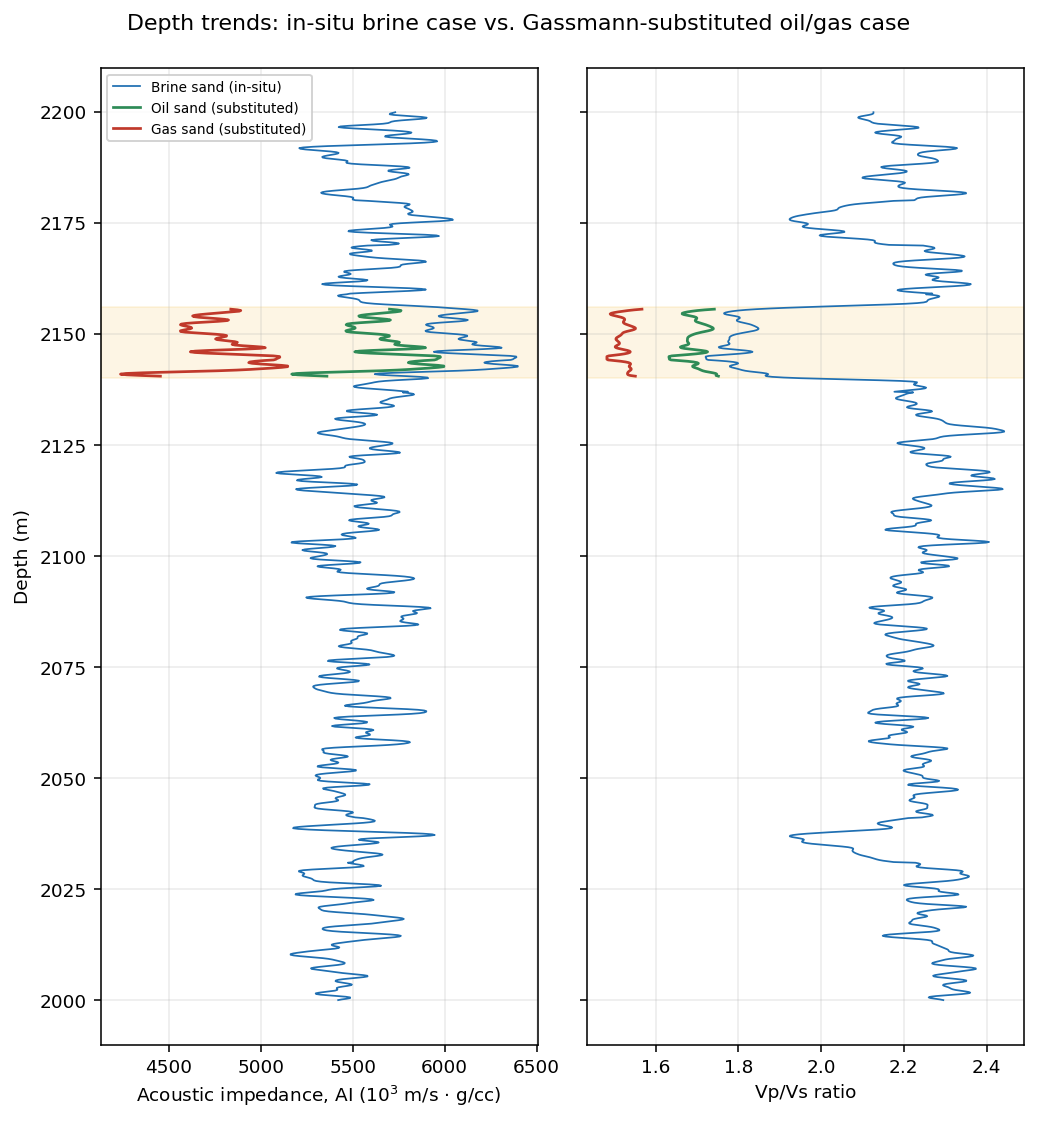
\includegraphics[width=0.75\textwidth]{02_depth_trends.png}
\caption{Depth trends of acoustic impedance and Vp/Vs ratio: in-situ brine case versus Gassmann-substituted oil and gas cases.}
\label{fig:trends}
\end{figure}

\subsection{Fluid Substitution Results}

Table~\ref{tab:reservoir} summarizes the average elastic properties of the clean reservoir interval (2142--2154~m, excluding the smoothed lithology-boundary transition zones) for each fluid case.

\begin{table}[htbp]
\centering
\caption{Reservoir sand elastic properties by fluid case (clean-interval average).}
\label{tab:reservoir}
\begin{tabular}{lcccccc}
\toprule
Fluid & \(V_p\) (m/s) & \(V_s\) (m/s) & \(\rho\) (g/cc) & AI & \(V_p/V_s\) \\
\midrule
Brine (in-situ) & 2929 & 1637 & 2.093 & 6131 & 1.790 \\
Oil (substituted) & 2804 & 1660 & 2.036 & 5709 & 1.690 \\
Gas (substituted) & 2681 & 1765 & 1.800 & 4826 & 1.519 \\
\bottomrule
\end{tabular}
\end{table}

Relative to the in-situ brine case, gas substitution reduces \(V_p\) by 8.5\%, bulk density by 14.0\%, and \(V_p/V_s\) by 15.1\% -- consistent with the well-established rock-physics signature of gas: the pore-fluid bulk modulus collapses far more than the rock frame changes, so \(K_\mathrm{sat}\) (and hence \(V_p\)) drops sharply while \(V_s\), which depends only on the fluid-insensitive shear modulus and the (comparatively modest) density change, is far less affected.

\subsection{Rock Physics Template and Lithofluid Discrimination}

Figure~\ref{fig:rpt} shows the calibrated rock physics template. The three sand trends (brine, oil, gas) separate cleanly in Vp/Vs-AI space at fixed porosity, and the shale trend sits at systematically higher Vp/Vs for a given impedance -- the classic basis for using this crossplot domain to discriminate both lithology and fluid type simultaneously. The well-log samples and synthetic core-plug measurements calibrate the reservoir-sand portion of the template well.

\begin{figure}[htbp]
\centering
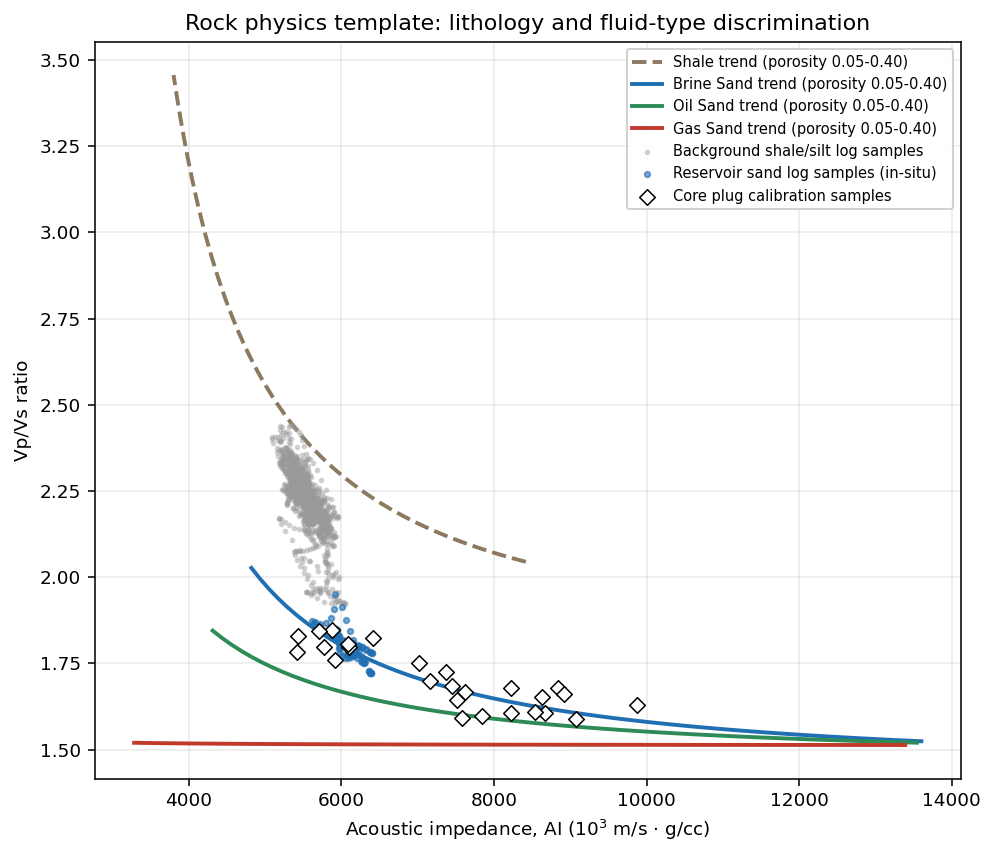
\includegraphics[width=0.75\textwidth]{03_rock_physics_template.png}
\caption{Rock physics template: Vp/Vs versus acoustic impedance, with brine/oil/gas-sand and shale trend lines, well-log samples, and synthetic core-plug calibration samples.}
\label{fig:rpt}
\end{figure}

Figure~\ref{fig:lmr} decomposes the same reservoir elastic states into the Lambda-Rho / Mu-Rho attribute domain (Goodway et al., 1997). Because Gassmann's formulation holds the shear modulus fluid-independent -- and \(\mu\rho \equiv \rho V_s^2 = \mu\) identically -- the brine, oil, and gas points fall at essentially the same \(\mu\rho\) while spreading widely in \(\lambda\rho\) (incompressibility). This is a direct, first-principles illustration of why the LMR domain is used industry-wide for fluid discrimination: it isolates the fluid-sensitive term from the fluid-insensitive one. Shale, having different mineralogy and frame properties, separates cleanly on the \(\mu\rho\) axis.

\begin{figure}[htbp]
\centering
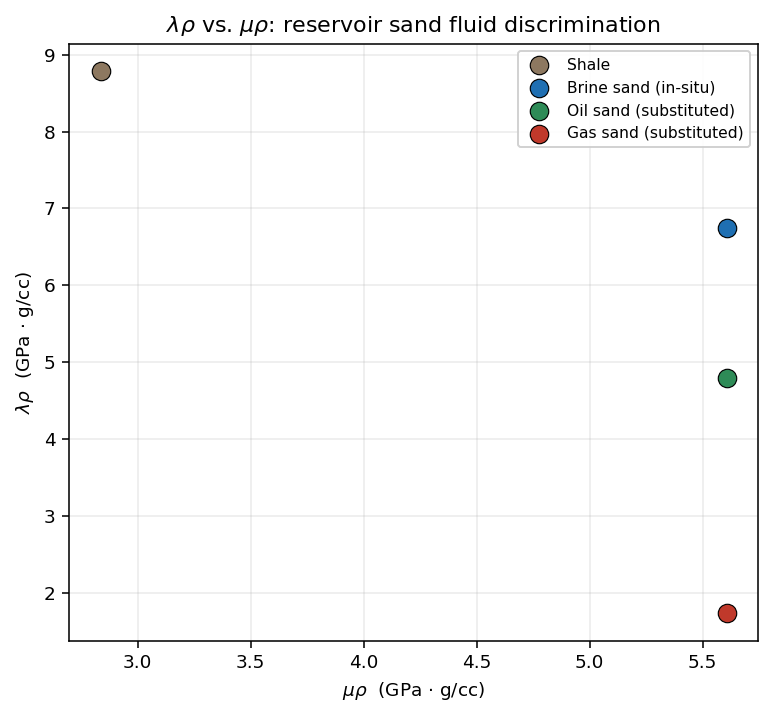
\includegraphics[width=0.6\textwidth]{04_lambda_mu_rho.png}
\caption{Lambda-Rho versus Mu-Rho: fluid discrimination in the reservoir sand, and lithology discrimination against the shale cap.}
\label{fig:lmr}
\end{figure}

Figure~\ref{fig:vpphi} shows the Vp-porosity domain, in which the compaction trend and fluid-substitution trend are visually distinguishable: samples move along the porosity axis primarily due to compaction, and drop vertically (at roughly constant porosity) due to fluid substitution.

\begin{figure}[htbp]
\centering
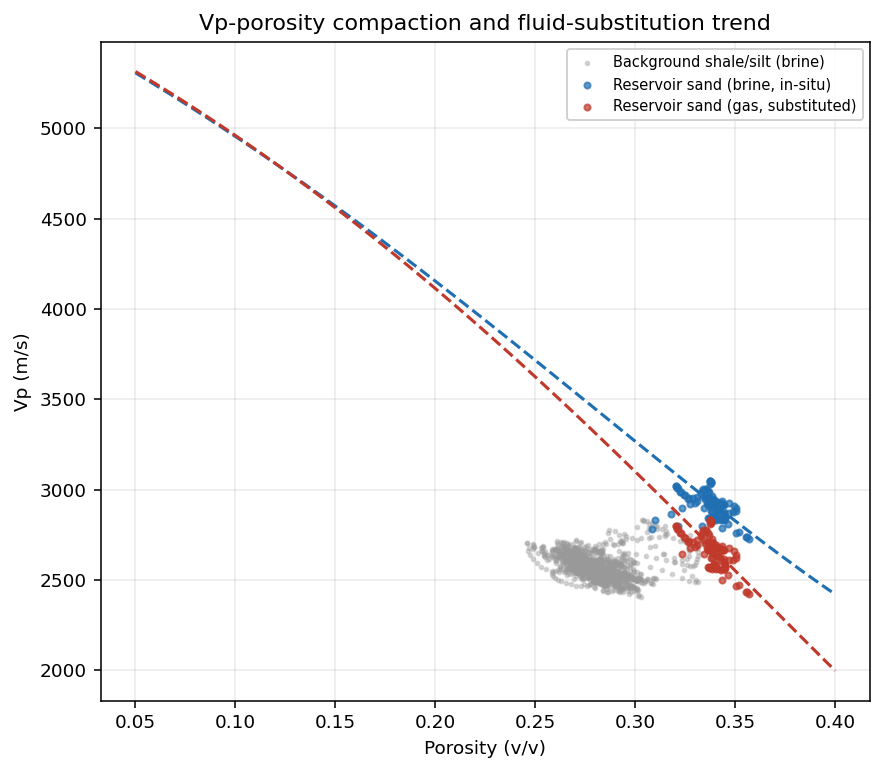
\includegraphics[width=0.65\textwidth]{05_vp_porosity.png}
\caption{Vp-porosity crossplot showing the compaction trend (background shale/silt) and the fluid-substitution offset between brine and gas cases in the reservoir sand.}
\label{fig:vpphi}
\end{figure}

\subsection{Synthetic AVO Gathers and Classification}

Figure~\ref{fig:gathers} shows the synthetic pre-stack angle gathers for the three fluid cases. The brine case shows a modest, single-polarity amplitude at the top-of-reservoir reflection; the oil case shows a markedly weaker near-offset response with amplitude building gradually with angle; the gas case shows a strong, clearly offset-dependent amplitude at both the top and base of the reservoir, with visible tuning interference between the two closely spaced (16~m) reflectors. Figure~\ref{fig:stacks} presents the corresponding near/mid/far stacks, and Figure~\ref{fig:crossplot} the intercept-gradient classification.

\begin{figure}[htbp]
\centering
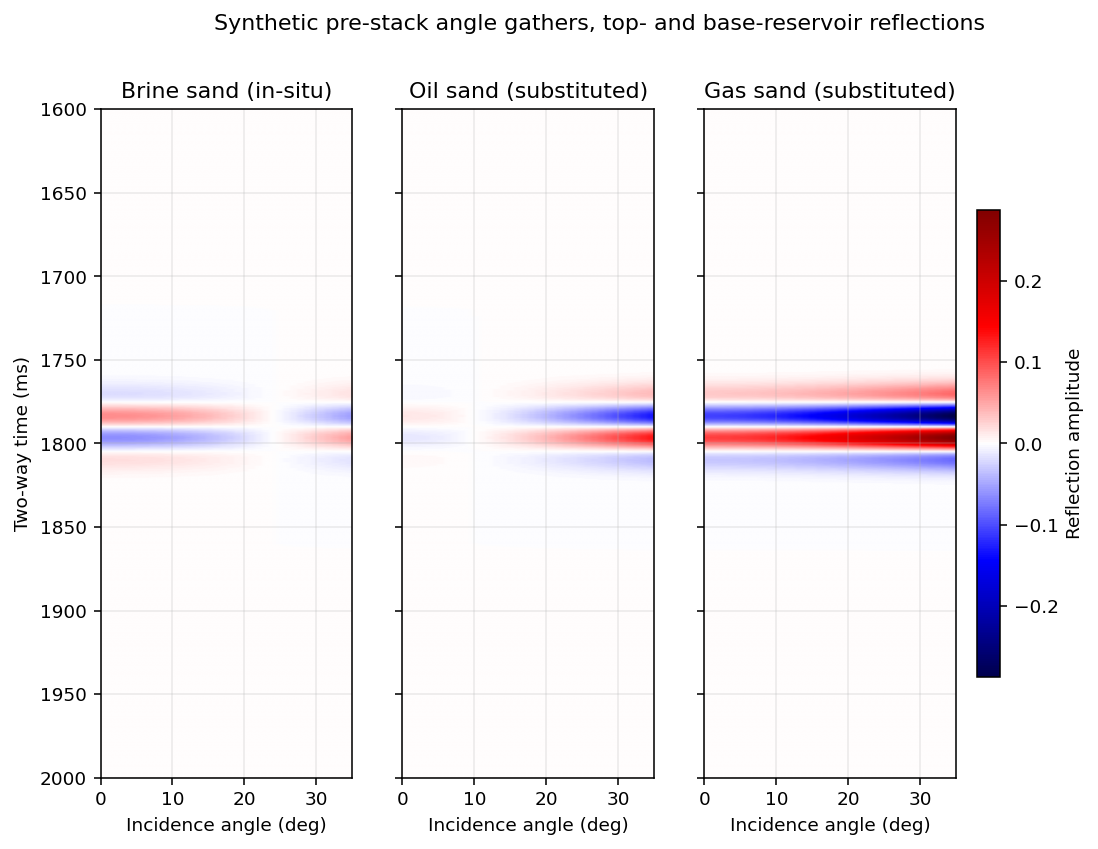
\includegraphics[width=\textwidth]{06_angle_gathers.png}
\caption{Synthetic pre-stack angle gathers (0--35\textdegree), top- and base-of-reservoir reflections, for the brine, oil, and gas cases.}
\label{fig:gathers}
\end{figure}

\begin{figure}[htbp]
\centering
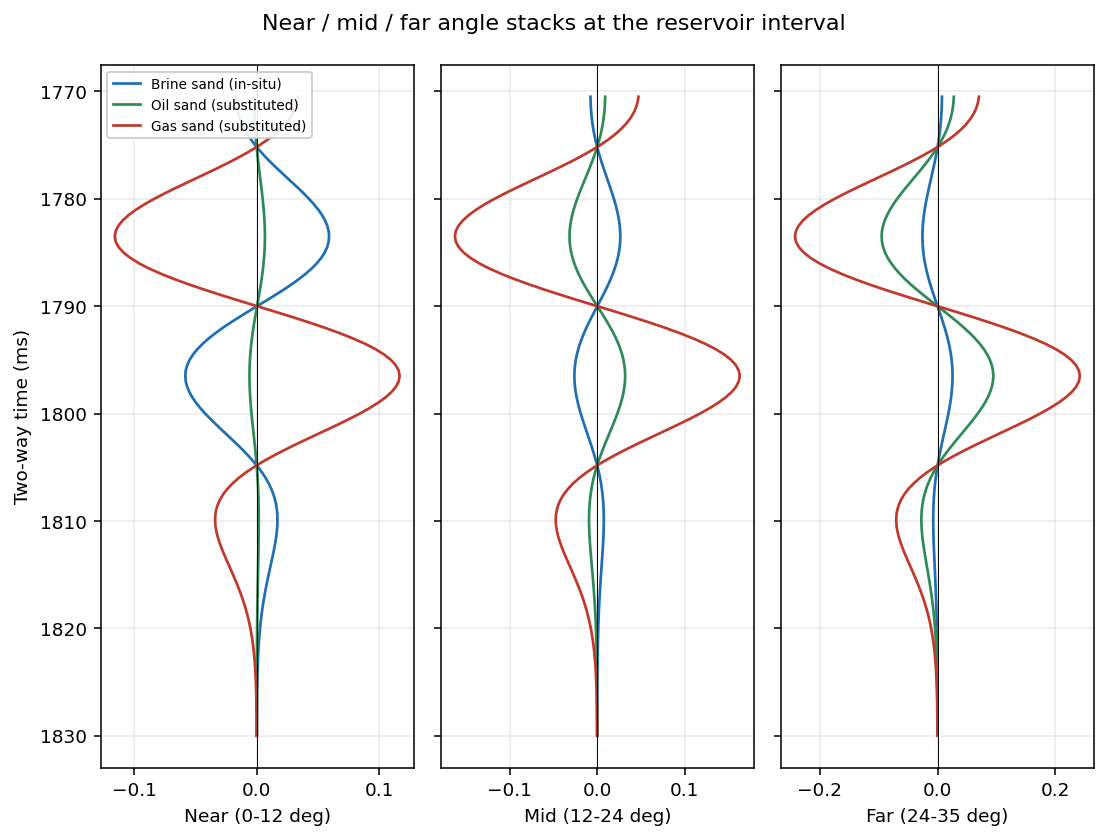
\includegraphics[width=0.7\textwidth]{07_near_mid_far_stacks.png}
\caption{Near, mid, and far angle stacks at the reservoir interval, by fluid case.}
\label{fig:stacks}
\end{figure}

\begin{figure}[htbp]
\centering
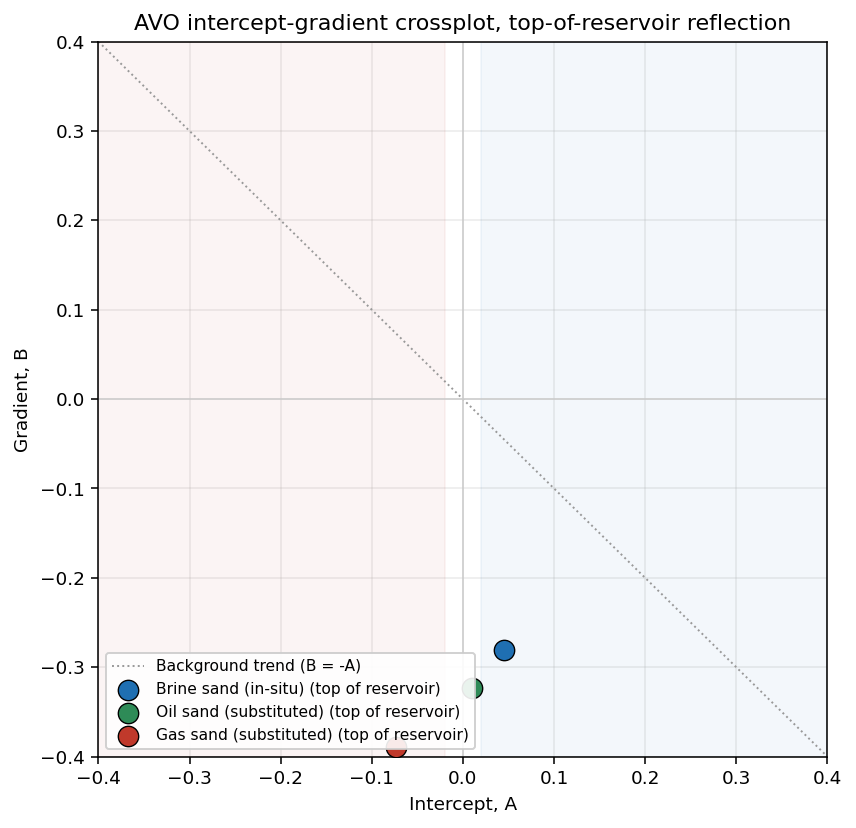
\includegraphics[width=0.62\textwidth]{08_avo_crossplot.png}
\caption{AVO intercept-gradient crossplot for the top-of-reservoir reflection, with Rutherford \& Williams (1989) / Castagna \& Swan (1997) class boundaries.}
\label{fig:crossplot}
\end{figure}

Table~\ref{tab:avo} summarizes the resulting classification. The brine case (\(A=+0.045\), \(B=-0.280\)) falls in Class~I territory: the in-situ sand is slightly stiffer (higher impedance) than the shale cap, giving a positive intercept whose amplitude weakens with offset. Substituting oil moves the intercept to \(A=+0.010\) -- within a few hundredths of zero -- while the gradient remains strongly negative; this is a genuinely subtle anomaly, straddling the Class~I/Class~II boundary, that would be difficult to identify from a near-offset stack alone and only becomes diagnostic once the far-offset amplitude and gradient are examined together. Gas substitution drives the response firmly into Class~III territory (\(A=-0.074\), \(B=-0.390\)): a classic unconsolidated-sand bright spot, with reflection amplitude growing markedly and unambiguously with offset.

\begin{table}[htbp]
\centering
\caption{AVO intercept/gradient classification, top-of-reservoir reflection.}
\label{tab:avo}
\begin{tabular}{lccl}
\toprule
Fluid & Intercept, \(A\) & Gradient, \(B\) & Classification \\
\midrule
Brine (in-situ) & +0.045 & $-$0.280 & Class I \\
Oil (substituted) & +0.010 & $-$0.324 & Class II / IIp (subtle) \\
Gas (substituted) & $-$0.074 & $-$0.390 & Class III (bright spot) \\
\bottomrule
\end{tabular}
\end{table}

\section{Discussion}

The workflow reproduces, from first principles, several well-established rock-physics and AVO relationships: the disproportionate sensitivity of \(V_p\) and \(V_p/V_s\) to gas relative to \(V_s\); the fluid-independence of the shear modulus (and hence of \(\mu\rho\)) under Gassmann's assumptions; and the progression from a Class~I in-situ response, through a subtle, near-zero-intercept Class~II/IIp anomaly for a moderate-impedance-contrast fluid case, to an unambiguous Class~III bright spot for gas. The oil case is arguably the most instructive result here: it demonstrates concretely why AVO interpretation requires examining the full-angle gradient rather than a single stack, since its near-zero intercept would be easy to overlook without gradient information.

Several simplifications should be kept in mind when applying this workflow's conclusions. The rock-physics model uses a uniform (Reuss-average, fully mixed) fluid saturation rather than a patchy-saturation model, which can meaningfully affect the seismic response at intermediate saturations. The oil and gas PVT properties are simplified representative relations rather than a full live-fluid Batzle-Wang treatment calibrated to a measured GOR and gas composition. The AVO modelling uses a linearized, weak-contrast reflectivity approximation valid to roughly 30--35\textdegree, and a 1D, normal-incidence-only wavelet convolution that does not capture offset-dependent tuning, NMO stretch, or anisotropy. None of these simplifications change the qualitative conclusions above, but a field application would need to revisit each of them against measured data.

\section{Conclusions}

\begin{enumerate}[label=(\arabic*)]
\item A first-principles Gassmann fluid-substitution workflow, applied to a synthetic shaly-sand Tertiary reservoir, correctly reproduces the expected asymmetric sensitivity of \(V_p\) and \(V_p/V_s\) to pore fluid, with gas substitution producing an 8.5\% reduction in \(V_p\) and a 15.1\% reduction in \(V_p/V_s\) relative to the in-situ brine case.
\item A Vp/Vs-versus-acoustic-impedance rock physics template, calibrated against synthetic log and core data, cleanly separates brine, oil, and gas sand trends from the shale background, and a Lambda-Rho/Mu-Rho decomposition of the same data directly illustrates the physical basis for that separation.
\item Pre-stack AVO modelling of the three fluid cases classifies the in-situ (brine) response as Class~I, the oil-substituted response as a subtle, near-zero-intercept Class~II/IIp anomaly, and the gas-substituted response as an unambiguous Class~III bright spot -- demonstrating both a clear-cut and a genuinely difficult fluid-discrimination scenario within a single, internally consistent reservoir model.
\item The complete workflow, from synthetic log construction through fluid substitution, rock-physics templating, and pre-stack AVO modelling, is implemented in openly available Python source code and is fully and deterministically reproducible.
\end{enumerate}

\newpage
\begin{thebibliography}{99}

\bibitem{aki1980} Aki, K., and Richards, P. G., 1980, \textit{Quantitative Seismology}. W. H. Freeman.

\bibitem{athy1930} Athy, L. F., 1930, Density, porosity, and compaction of sedimentary rocks. \textit{AAPG Bulletin}, 14, 1--24.

\bibitem{batzle1992} Batzle, M., and Wang, Z., 1992, Seismic properties of pore fluids. \textit{Geophysics}, 57(11), 1396--1408.

\bibitem{castagna1997} Castagna, J. P., and Swan, H. W., 1997, Principles of AVO crossplotting. \textit{The Leading Edge}, 16(4), 337--342.

\bibitem{gassmann1951} Gassmann, F., 1951, \"Uber die Elastizit\"at por\"oser Medien. \textit{Vierteljahrsschrift der Naturforschenden Gesellschaft in Z\"urich}, 96, 1--23.

\bibitem{goodway1997} Goodway, B., Chen, T., and Downton, J., 1997, Improved AVO fluid detection and lithology discrimination using Lambda-Mu-Rho (LMR). \textit{67th SEG Annual Meeting, Expanded Abstracts}.

\bibitem{hill1952} Hill, R., 1952, The elastic behaviour of a crystalline aggregate. \textit{Proceedings of the Physical Society. Section A}, 65(5), 349--354.

\bibitem{krief1990} Krief, M., Garat, J., Stellingwerff, J., and Ventre, J., 1990, A petrophysical interpretation using the velocities of P and S waves (full waveform sonic). \textit{The Log Analyst}, 31, 355--369.

\bibitem{mavko2009} Mavko, G., Mukerji, T., and Dvorkin, J., 2009, \textit{The Rock Physics Handbook}, 2nd ed. Cambridge University Press.

\bibitem{rutherford1989} Rutherford, S. R., and Williams, R. H., 1989, Amplitude-versus-offset variations in gas sands. \textit{Geophysics}, 54(6), 680--688.

\bibitem{shuey1985} Shuey, R. T., 1985, A simplification of the Zoeppritz equations. \textit{Geophysics}, 50(4), 609--614.

\end{thebibliography}

\end{document}
